\section{Variational Autoencoders (VAEs)}
\label{VAEs}

A questo punto si è giunti finalmente al cuore di questa trattazione, dove vengono illustrate le basi teoriche di un metodo di apprendimento non supervisionato, il Variational Autoencoders (VAEs), del quale si studierà nella prossima sezione un'applicazione al campo della fisica delle alte energie. \\
Il percorso seguito in questa sezione è il seguente:
\begin{itemize}
	\item Problema della dimensionalità;
	\item Autoencoders;
	\item Variational Autoencoders.
\end{itemize}

\subsection{Curse of dimensionality e riduzione della dimensionalità}
\label{curse_dim}

Come è stato più volte detto in questa trattazione, quando si parla di input (o pattern) ci si riferisce a dei vettori, le cui componenti sono i dati veri e propri; questi vettori, in quanto tali, possono essere pensati all'interno di un opportuno spazio n-dimensionale (con n=numero di componenti del vettore).\\
Quando si parla di "Curse of dimensionality" (letteralmente "la maledizione della dimensionalità") ci si riferisce ad una serie di problemi che ci si trova ad affrontare quando bisogna trattare spazi con un'alta dimensionalità, che altrimenti non comparirebbero in spazi a bassa dimensionalità.  \\
Dato che all'aumentare della dimensionalità i volumi nello spazio aumentano in maniera significativa, ci si troverà nella situazione per cui i pattern risultano sparsi nello spazio e questo è chiaramente un problema per ogni analisi che ne si vuole fare basata sulla statistica; infatti, per ottenere dei risultati significativi a livello statistico, la quantità di dati necessari aumenta in maniera esponenziale e questo risulta essere un problema a livello pratico. \\
Quando si parla di riduzione della dimensionalità ci si riferisce ad una serie di tecniche, attraverso le quali viene ridotto il numero delle variabili che caratterizzano i vettori di input; l'obiettivo di base è quello di proiettare gli elementi dello spazio n-dimensionale (i vettori di input) su di uno spazio a dimensione inferiore, cogliendo l'essenza stessa dei dati.\\
Ciò che è necessario notare è che avere degli input con più bassa dimensionalità permette di avere anche meno parametri (gradi di libertà) e quindi una struttura più semplice del modello. Il prediligere la semplicità alla complessità, oltre che per gli ovvi motivi, deriva dal fatto che la seconda è molto soggetta al fenomeno dell'overfitting. \\
Il processo di riduzione della dimensionalità è una metodologia di preparazione dei dati, per poi essere presentati all'algoritmo di apprendimento, che si troverà di fronte delle informazioni più compatte e quindi più facilmente processabili. \\
Inoltre bisogna notare che, se il processo di riduzione della dimensionalità viene svolto sul training data set, allora deve essere attuato anche sul test data set, per garantire un processo di verifica valido.
\newpage

Il processo di riduzione della dimensionalità può essere portato avanti attraverso due metodologie differenti:
\begin{itemize}
	\item Selezione, dove solo alcune componenti dei vettori di input vengono conservate;
	\item Estrazione, dove viene creato un numero ridotto di nuove componenti a partire da quelle originali.
\end{itemize}
A prescindere da questa distinzione, bisogna sottolineare che tutti i processi di riduzione della dimensionalità hanno una struttura comune, ovvero sono caratterizzati da una fase di $\textit{encoding}$ (che rappresenta il vero e proprio processo di riduzione della dimensionalità) e da una fase di $\textit{decoding}$, nella quale si verifica quanta informazione è stata persa nel processo. \\ 
Si riporta in figura ~\ref{encoder-decoder} l'illustrazione grafica del processo $\textit{encoding-decoding}$
\begin{figure}[h!]
	\centering
	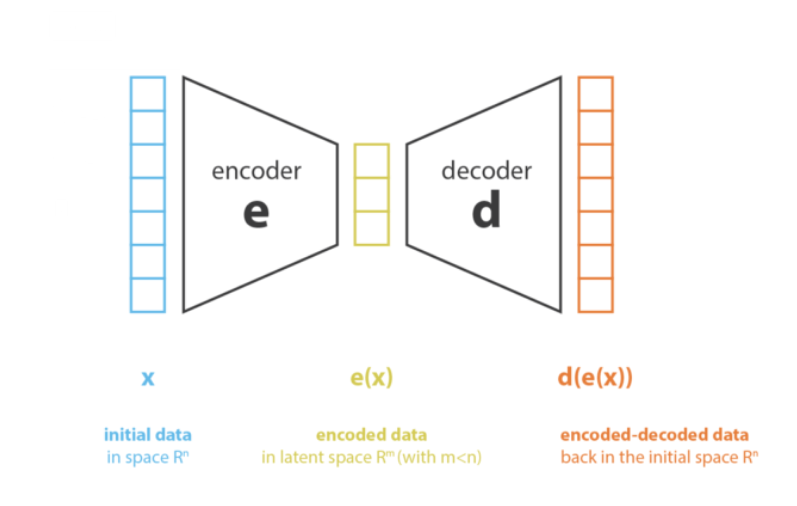
\includegraphics[width=0.90\textwidth]{figs/encoder-decoder.png}
	\caption{Strutture generale di un processo di riduzione della dimensionalità . L'immagine è presa da \cite{Understanding_VAEs}}
	\label{encoder-decoder}
\end{figure}

Il vettore di input $\textbf{x}$ (n-dimensionale) viene compresso dall'encoder $\textbf{e}$ in un vettore $\textbf{e}(\textbf{x})$ di uno spazio m-dimensionale (con m<n), detto $\textit{spazio latente}$; l'encoder, come detto, può agire per selezione o per estrazione. \\
Il decoder $\textbf{d}$ svolge la funzione opposta, ovvero decomprime il vettore $\textbf{e}(\textbf{x})$ in $\textbf{d}(\textbf{e}(\textbf{x}))$ per tornare allo spazio originario n-dimensionale. \\
Nel caso in cui $\textbf{x} = \textbf{d}(\textbf{e}(\textbf{x}))$ (caso ideale) si dice che il processo è un $\textit{lossless encoding}$, ovvero non c'è stata perdita di informazioni nella riduzione della dimensionalità; viceversa, se $\textbf{x} \not= \textbf{d}(\textbf{e}(\textbf{x}))$, si parla di un $\textit{lossy encoding}$, cioè un processo nel quale parte dell'informazione viene persa e non può essere recuperata con la fase di decoding. \\
\newpage
Come conseguenza di ciò che è stato appena illustrato, l'obiettivo di un processo di riduzione della dimensionalità è quello di trovare la coppia encoder-decoder (e,d) fra una famiglia di encoder E e di decoder D, che minimizzi l'informazione persa:
\begin{equation}
	(e,d) = \min_{E \times D} \epsilon (\textbf{x},\textbf{d}(\textbf{e}(\textbf{x})))
\end{equation}
dove $\epsilon (\textbf{x},\textbf{d}(\textbf{e}(\textbf{x})))$ è la grandezza attraverso la quale viene  quantificata la quantità di informazione persa nel processo di riduzione. \\ \\
A questo punto è possibile illustrare le varie metodologie di riduzione della dimensionalità, secondo la distinzione già incontrata fra selezione ed estrazione. \\
I metodi di selezione ("Feature Selection Methods (FSM)") sono metodi attraverso i quali vengono selezionate le componenti dei vettori di input da tenere e quelle da eliminare perché irrilevanti per le analisi successive; a proposito dei 